The original paper \supercite{Geisshirt:1997} was published as part of my
PhD thesis \supercite{Geisshirt:PhD}. The research was carried out in the
last decade of the 20th century. My research interest was in the cross-disiplinary
field of non-equilibrium statistical thermodynamics, chemical kinetics, and
complexity theory.

In the 1990s, computers were reliable and accessible. Growing up with home computers
the decade before, they were regarded as scientific calculators - at least to me.
An eternal truth for scientists is that they must carry out their research at
the boundary of what is possible. The emerging field of computational science
was not an exception, I simulated only system at the edge of what computational capacity
which was accessible. UNIX workstations and supercomputers were an integral
part of my daily life.

\subsection{Short summary of research}

My PhD research involved a number of smaller projects, and in the paper in focus
for this reproduction study, my supervisors and I went out of a quest to
find a simple model for oscillating chemical reactions. During the 1970s and 1980s,
oscillating chemical reactions were studies experimentally and modelled
mathematically. The mathematical models were on macroscopic level, and
chemical reactions far from equilibrium were linked to complexity theory and
chaos theory \supercite{Kuramoto:1984} \supercite{Prigogine:1984} \supercite{Nicolis:1989}.

Instead of modelling on the macroscopic level, we investigated chemical reactions at
a microscopic level. Simple molecules (single particles) were simulated
using classical mechanics. The Lennard-Jones (LJ) potential is known to behave as
simple liquids. Tuning the LJ parameters, a phase transition can be observed.

The original paper sets the scene of a mixture of three diffferent kind of particles
($A$, $B$, and $C$). When a pair of odd particles (e.g., $A$ and $B$) are close,
a chemical reaction happens with a given probability. We studies three reactions:

\begin{eqnarray}
    A + B &\rightarrow 2B \\
    B + C &\rightarrow 2C \\
    C + A &\rightarrow 2A
\end{eqnarray}

This is a simple extension of the well-known Volterra-Lotka mechanism
\supercite{Lotka:1910} \supercite{Lotka:1920}.

In the original paper, we demonstrate that it is possible to observe oscillating
chemical reactions. Moreover, above the critical temperature (at $\rho = 0.8$,
the critical temperature $T_c \approx 1.8$ on a unitless scale), the
mixture is homogenous, while below the critical temperature,
a phase seperation will occur and a heterogeous state will emerge.

Calculating instantenous rate constants ($k$) for the three reacting is done by
counting the number of reaction events, and the diffusion coefficient ($D$)
can be calculated using mean displacement. The main result of the original
paper is that when the plotting $k/D$ vs. temperature, the phase transition can
be observe.

\subsection{Original hardware and its limitations}

In the 1990s, computers were reliable but limited in capacity (for computational scientists,
computers will always have limited capacity). As a PhD student, I was fortunate to
have an IBM RS/6000 workstation with a PowerPC 601 CPU. I cannot recall the exact specifications,
but clock frequency was not higher than 100 MHz. The size of the memory was in the order
of 16 MB or 32 MB, and the operating system was AIX.

At the Danish supercomputer centre (UNI-C), an IBM SP was installed in 1994 \supercite{Hultberg:1999}.
In order to run long simulations or large system (65536 particles), I used the IBM SP.
All postprocessing and data analysis done on my local IBM workstation.

\subsection{Building software}

The software used for the simulations is written in Fortran-77. I have kept a copy (first
on a floppy disk, later on an USB stick and finally in a Github repository). It consists of
only a couple of files, and a simple Makefile can be used.

Building the software on Debian GNU/Linux 9 and MacOS 10.15 is still possible. GNU Fortran
(part of GNU Compiler Collection) can easily compile the source files and linked
the software to a final binary. Only minor changes were required - mostly to the
flags used by GNU Fortran compared to AIX Fortran.

Unfortunately, software to calculate rate constants and diffusion coefficients were lost.
From the description in my PhD thesis \supercite{Geisshirt:PhD} I was able to rewrite it.
This time I rewrote the piece in Python giving me an excuse to play with Numpy.

\subsection{Findings}

From the original \LaTeX files of my PhD thesis (also archived as a Github repository),
I had access to the data for figure 6 in the original paper. To reproduce the data,
simulations at a temperature range were carried out.

Two decades ago I used a supercomputer to do the simulations, but for this
reproduction study I used a much smaller computer: A small Debian GNU/Linux
based computer (Intel Atom D2700 at 2.13 MHz and 8 GB memory). With so much
computing power, I could not resist the temptation to double the
number of simulations (18 vs. 42).

In figure \ref{kD} the original data and the new data are displayed together.
The two data sets are similar, and the phase transition at $T \approx 1.8$
can be observed.


\begin{figure}
    \label{kD}
    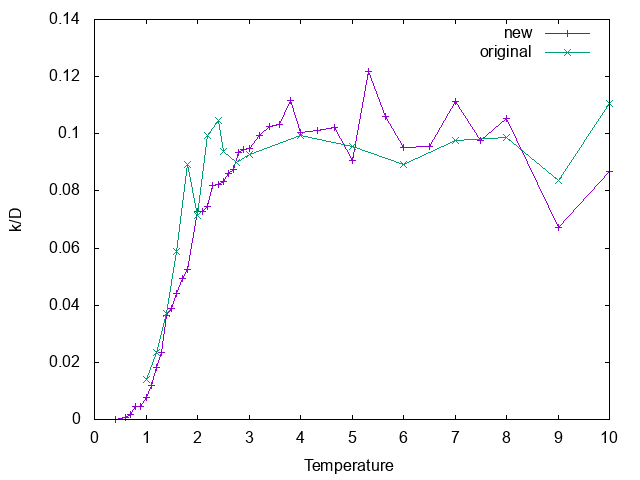
\includegraphics{kD.png}
\end{figure}
